\documentclass[1p]{elsarticle_modified}
%\bibliographystyle{elsarticle-num}

%\usepackage[colorlinks]{hyperref}
%\usepackage{abbrmath_seonhwa} %\Abb, \Ascr, \Acal ,\Abf, \Afrak
\usepackage{amsfonts}
\usepackage{amssymb}
\usepackage{amsmath}
\usepackage{amsthm}
\usepackage{scalefnt}
\usepackage{amsbsy}
\usepackage{kotex}
\usepackage{caption}
\usepackage{subfig}
\usepackage{color}
\usepackage{graphicx}
\usepackage{xcolor} %% white, black, red, green, blue, cyan, magenta, yellow
\usepackage{float}
\usepackage{setspace}
\usepackage{hyperref}

\usepackage{tikz}
\usetikzlibrary{arrows}

\usepackage{multirow}
\usepackage{array} % fixed length table
\usepackage{hhline}

%%%%%%%%%%%%%%%%%%%%%
\makeatletter
\renewcommand*\env@matrix[1][\arraystretch]{%
	\edef\arraystretch{#1}%
	\hskip -\arraycolsep
	\let\@ifnextchar\new@ifnextchar
	\array{*\c@MaxMatrixCols c}}
\makeatother %https://tex.stackexchange.com/questions/14071/how-can-i-increase-the-line-spacing-in-a-matrix
%%%%%%%%%%%%%%%

\usepackage[normalem]{ulem}

\newcommand{\msout}[1]{\ifmmode\text{\sout{\ensuremath{#1}}}\else\sout{#1}\fi}
%SOURCE: \msout is \stkout macro in https://tex.stackexchange.com/questions/20609/strikeout-in-math-mode

\newcommand{\cancel}[1]{
	\ifmmode
	{\color{red}\msout{#1}}
	\else
	{\color{red}\sout{#1}}
	\fi
}

\newcommand{\add}[1]{
	{\color{blue}\uwave{#1}}
}

\newcommand{\replace}[2]{
	\ifmmode
	{\color{red}\msout{#1}}{\color{blue}\uwave{#2}}
	\else
	{\color{red}\sout{#1}}{\color{blue}\uwave{#2}}
	\fi
}

\newcommand{\Sol}{\mathcal{S}} %segment
\newcommand{\D}{D} %diagram
\newcommand{\A}{\mathcal{A}} %arc


%%%%%%%%%%%%%%%%%%%%%%%%%%%%%5 test

\def\sl{\operatorname{\textup{SL}}(2,\Cbb)}
\def\psl{\operatorname{\textup{PSL}}(2,\Cbb)}
\def\quan{\mkern 1mu \triangleright \mkern 1mu}

\theoremstyle{definition}
\newtheorem{thm}{Theorem}[section]
\newtheorem{prop}[thm]{Proposition}
\newtheorem{lem}[thm]{Lemma}
\newtheorem{ques}[thm]{Question}
\newtheorem{cor}[thm]{Corollary}
\newtheorem{defn}[thm]{Definition}
\newtheorem{exam}[thm]{Example}
\newtheorem{rmk}[thm]{Remark}
\newtheorem{alg}[thm]{Algorithm}

\newcommand{\I}{\sqrt{-1}}
\begin{document}

%\begin{frontmatter}
%
%\title{Boundary parabolic representations of knots up to 8 crossings}
%
%%% Group authors per affiliation:
%\author{Yunhi Cho} 
%\address{Department of Mathematics, University of Seoul, Seoul, Korea}
%\ead{yhcho@uos.ac.kr}
%
%
%\author{Seonhwa Kim} %\fnref{s_kim}}
%\address{Center for Geometry and Physics, Institute for Basic Science, Pohang, 37673, Korea}
%\ead{ryeona17@ibs.re.kr}
%
%\author{Hyuk Kim}
%\address{Department of Mathematical Sciences, Seoul National University, Seoul 08826, Korea}
%\ead{hyukkim@snu.ac.kr}
%
%\author{Seokbeom Yoon}
%\address{Department of Mathematical Sciences, Seoul National University, Seoul, 08826,  Korea}
%\ead{sbyoon15@snu.ac.kr}
%
%\begin{abstract}
%We find all boundary parabolic representation of knots up to 8 crossings.
%
%\end{abstract}
%\begin{keyword}
%    \MSC[2010] 57M25 
%\end{keyword}
%
%\end{frontmatter}

%\linenumbers
%\tableofcontents
%
\newcommand\colored[1]{\textcolor{white}{\rule[-0.35ex]{0.8em}{1.4ex}}\kern-0.8em\color{red} #1}%
%\newcommand\colored[1]{\textcolor{white}{ #1}\kern-2.17ex	\textcolor{white}{ #1}\kern-1.81ex	\textcolor{white}{ #1}\kern-2.15ex\color{red}#1	}

{\Large $\underline{8_{16}~(K8a_{15})}$}

\setlength{\tabcolsep}{10pt}
\renewcommand{\arraystretch}{1.6}
\vspace{1cm}\begin{tabular}{m{100pt}>{\centering\arraybackslash}m{274pt}}
\multirow{5}{120pt}{
	\centering
	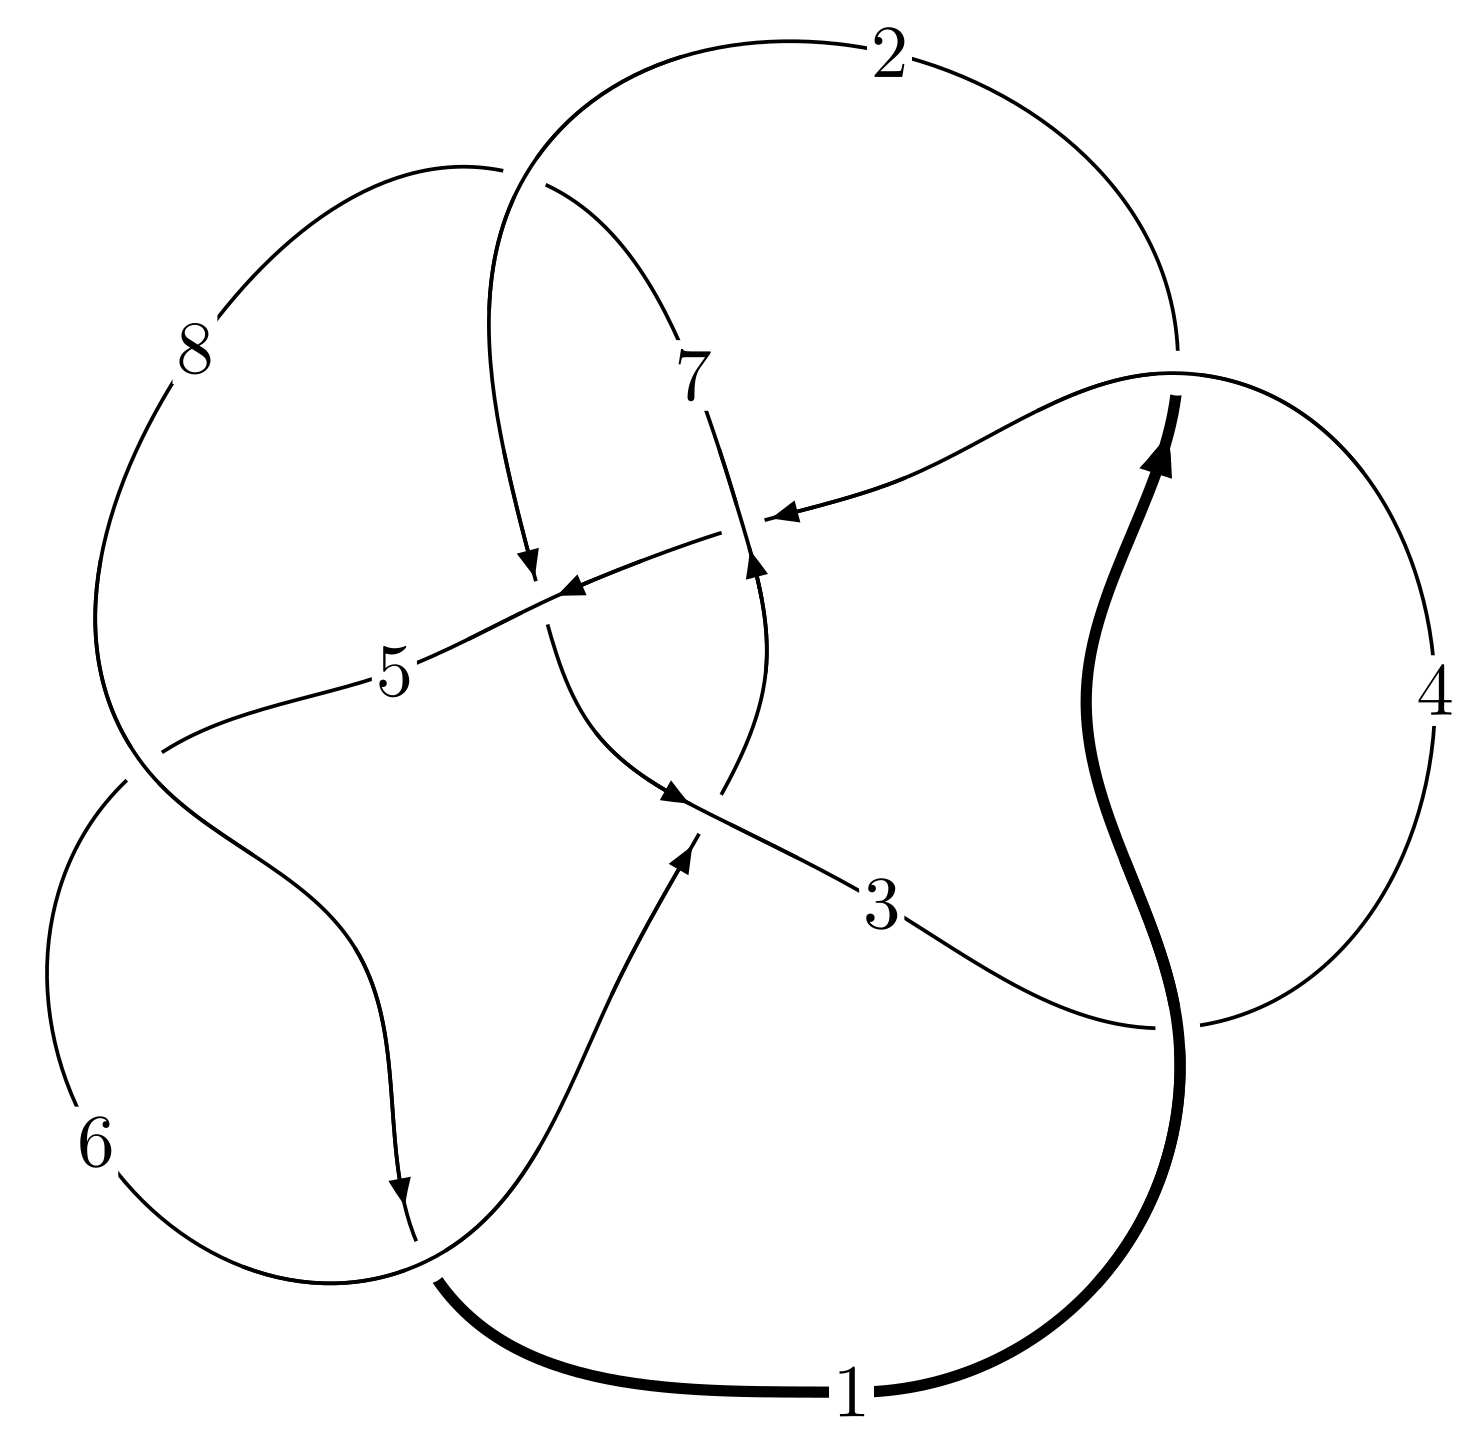
\includegraphics[width=112pt]{../../../GIT/diagram.site/Diagrams/png/30_8_16.png}\\
\ \ \ A knot diagram\footnotemark}&
\allowdisplaybreaks
\textbf{Linearized knot diagam} \\
\cline{2-2}
 &
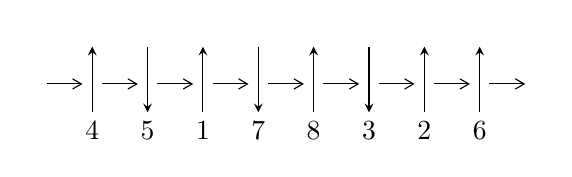
\begin{tikzpicture}[x=20pt, y=17pt]
	% nodes
	\node (C0) at (0, 0) {};
	\node (C1) at (1, 0) {};
	\node (C1U) at (1, +1) {};
	\node (C1D) at (1, -1) {4};

	\node (C2) at (2, 0) {};
	\node (C2U) at (2, +1) {};
	\node (C2D) at (2, -1) {5};

	\node (C3) at (3, 0) {};
	\node (C3U) at (3, +1) {};
	\node (C3D) at (3, -1) {1};

	\node (C4) at (4, 0) {};
	\node (C4U) at (4, +1) {};
	\node (C4D) at (4, -1) {7};

	\node (C5) at (5, 0) {};
	\node (C5U) at (5, +1) {};
	\node (C5D) at (5, -1) {8};

	\node (C6) at (6, 0) {};
	\node (C6U) at (6, +1) {};
	\node (C6D) at (6, -1) {3};

	\node (C7) at (7, 0) {};
	\node (C7U) at (7, +1) {};
	\node (C7D) at (7, -1) {2};

	\node (C8) at (8, 0) {};
	\node (C8U) at (8, +1) {};
	\node (C8D) at (8, -1) {6};
	\node (C9) at (9, 0) {};

	% arrows
	\draw[->,>={angle 60}]
	(C0) edge (C1) (C1) edge (C2) (C2) edge (C3) (C3) edge (C4) (C4) edge (C5) (C5) edge (C6) (C6) edge (C7) (C7) edge (C8) (C8) edge (C9) ;	\draw[->,>=stealth]
	(C1D) edge (C1U) (C2U) edge (C2D) (C3D) edge (C3U) (C4U) edge (C4D) (C5D) edge (C5U) (C6U) edge (C6D) (C7D) edge (C7U) (C8D) edge (C8U) ;
	\end{tikzpicture} \\
\hhline{~~} \\& 
\textbf{Solving Sequence} \\ \cline{2-2} 
 &
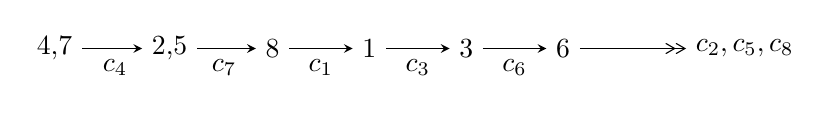
\begin{tikzpicture}[x=35pt, y=7pt]
	% node
	\node (A0) at (-1/8, 0) {4,7};
	\node (A1) at (17/16, 0) {2,5};
	\node (A2) at (17/8, 0) {8};
	\node (A3) at (25/8, 0) {1};
	\node (A4) at (33/8, 0) {3};
	\node (A5) at (41/8, 0) {6};
	\node (C1) at (1/2, -1) {$c_{4}$};
	\node (C2) at (13/8, -1) {$c_{7}$};
	\node (C3) at (21/8, -1) {$c_{1}$};
	\node (C4) at (29/8, -1) {$c_{3}$};
	\node (C5) at (37/8, -1) {$c_{6}$};
	\node (A6) at (7, 0) {$c_{2},c_{5},c_{8}$};

	% edge
	\draw[->,>=stealth]	
	(A0) edge (A1) (A1) edge (A2) (A2) edge (A3) (A3) edge (A4) (A4) edge (A5) ;
	\draw[->>,>={angle 60}]	
	(A5) edge (A6);
\end{tikzpicture} \\ 

\end{tabular} \\

\footnotetext{
The image of knot diagram is generated by the software ``\textbf{Draw programme}" developed by Andrew Bartholomew(\url{http://www.layer8.co.uk/maths/draw/index.htm\#Running-draw}), where we modified some parts for our purpose(\url{https://github.com/CATsTAILs/LinksPainter}).
}\phantom \\ \newline 
\centering \textbf{Ideals for irreducible components\footnotemark of $X_{\text{par}}$} 
 
\begin{align*}
I^u_{1}&=\langle 
- u^4+b+2 u-2,\;-5 u^4-2 u^3- u^2+a+10 u-11,\;u^5-2 u^2+3 u-1\rangle \\
I^u_{2}&=\langle 
816 u^{11}+1706 u^{10}+\cdots+605 b-492,\;-596 u^{11}-1838 u^{10}+\cdots+121 a-1235,\\
\phantom{I^u_{2}}&\phantom{= \langle  }u^{12}+3 u^{11}+6 u^{10}+9 u^9+20 u^8+31 u^7+41 u^6+39 u^5+34 u^4+22 u^3+12 u^2+4 u+1\rangle \\
\\
\end{align*}
\raggedright * 2 irreducible components of $\dim_{\mathbb{C}}=0$, with total 17 representations.\\
\footnotetext{All coefficients of polynomials are rational numbers. But the coefficients are sometimes approximated in decimal forms when there is not enough margin.}
\newpage
\renewcommand{\arraystretch}{1}
\centering \section*{I. $I^u_{1}= \langle - u^4+b+2 u-2,\;-5 u^4-2 u^3- u^2+a+10 u-11,\;u^5-2 u^2+3 u-1 \rangle$}
\flushleft \textbf{(i) Arc colorings}\\
\begin{tabular}{m{7pt} m{180pt} m{7pt} m{180pt} }
\flushright $a_{4}=$&$\begin{pmatrix}1\\0\end{pmatrix}$ \\
\flushright $a_{7}=$&$\begin{pmatrix}0\\u\end{pmatrix}$ \\
\flushright $a_{2}=$&$\begin{pmatrix}5 u^4+2 u^3+u^2-10 u+11\\u^4-2 u+2\end{pmatrix}$ \\
\flushright $a_{5}=$&$\begin{pmatrix}1\\u^2\end{pmatrix}$ \\
\flushright $a_{8}=$&$\begin{pmatrix}17 u^4+8 u^3+4 u^2-33 u+36\\3 u^4+u^3+u^2-5 u+6\end{pmatrix}$ \\
\flushright $a_{1}=$&$\begin{pmatrix}4 u^4+2 u^3+u^2-8 u+9\\u^4-2 u+2\end{pmatrix}$ \\
\flushright $a_{3}=$&$\begin{pmatrix}5 u^4+2 u^3+u^2-9 u+11\\u^4+u^3-2 u+2\end{pmatrix}$ \\
\flushright $a_{6}=$&$\begin{pmatrix}19 u^4+9 u^3+4 u^2-35 u+40\\3 u^4+2 u^3+u^2-6 u+7\end{pmatrix}$\\&\end{tabular}
\flushleft \textbf{(ii) Obstruction class $= -1$}\\~\\
\flushleft \textbf{(iii) Cusp Shapes $= -12 u^4-4 u^3+20 u-26$}\\~\\
\newpage\renewcommand{\arraystretch}{1}
\flushleft \textbf{(iv) u-Polynomials at the component}\newline \\
\begin{tabular}{m{50pt}|m{274pt}}
Crossings & \hspace{64pt}u-Polynomials at each crossing \\
\hline $$\begin{aligned}c_{1},c_{3},c_{5}\\c_{8}\end{aligned}$$&$\begin{aligned}
&u^5+2 u^4-2 u^2- u-1
\end{aligned}$\\
\hline $$\begin{aligned}c_{2},c_{4}\end{aligned}$$&$\begin{aligned}
&u^5+2 u^2+3 u+1
\end{aligned}$\\
\hline $$\begin{aligned}c_{6}\end{aligned}$$&$\begin{aligned}
&u^5+7 u^4+19 u^3+30 u^2+24 u+8
\end{aligned}$\\
\hline $$\begin{aligned}c_{7}\end{aligned}$$&$\begin{aligned}
&u^5+7 u^4+18 u^3+23 u^2+14 u+4
\end{aligned}$\\
\hline
\end{tabular}\\~\\
\newpage\renewcommand{\arraystretch}{1}
\flushleft \textbf{(v) Riley Polynomials at the component}\newline \\
\begin{tabular}{m{50pt}|m{274pt}}
Crossings & \hspace{64pt}Riley Polynomials at each crossing \\
\hline $$\begin{aligned}c_{1},c_{3},c_{5}\\c_{8}\end{aligned}$$&$\begin{aligned}
&y^5-4 y^4+6 y^3-3 y-1
\end{aligned}$\\
\hline $$\begin{aligned}c_{2},c_{4}\end{aligned}$$&$\begin{aligned}
&y^5+6 y^3-4 y^2+5 y-1
\end{aligned}$\\
\hline $$\begin{aligned}c_{6}\end{aligned}$$&$\begin{aligned}
&y^5-11 y^4-11 y^3-100 y^2+96 y-64
\end{aligned}$\\
\hline $$\begin{aligned}c_{7}\end{aligned}$$&$\begin{aligned}
&y^5-13 y^4+30 y^3-81 y^2+12 y-16
\end{aligned}$\\
\hline
\end{tabular}\\~\\
\newpage\flushleft \textbf{(vi) Complex Volumes and Cusp Shapes}
$$\begin{array}{c|c|c}  
\text{Solutions to }I^u_{1}& \I (\text{vol} + \sqrt{-1}CS) & \text{Cusp shape}\\
 \hline 
\begin{aligned}
u &= \phantom{-}0.761218 + 0.545187 I \\
a &= \phantom{-}0.148341 - 0.707998 I \\
b &= -0.131705 - 0.621876 I\end{aligned}
 & -1.32133 - 1.30034 I & -2.51370 + 2.13902 I \\ \hline\begin{aligned}
u &= \phantom{-}0.761218 - 0.545187 I \\
a &= \phantom{-}0.148341 + 0.707998 I \\
b &= -0.131705 + 0.621876 I\end{aligned}
 & -1.32133 + 1.30034 I & -2.51370 - 2.13902 I \\ \hline\begin{aligned}
u &= \phantom{-}0.476529\phantom{ +0.000000I} \\
a &= \phantom{-}6.93603\phantom{ +0.000000I} \\
b &= \phantom{-}1.09851\phantom{ +0.000000I}\end{aligned}
 & \phantom{-}3.68417\phantom{ +0.000000I} & -17.5210\phantom{ +0.000000I} \\ \hline\begin{aligned}
u &= -0.99948 + 1.18099 I \\
a &= -0.116359 - 1.043350 I \\
b &= -1.41755 - 0.49337 I\end{aligned}
 & \phantom{-}6.88145 + 10.57900 I & \phantom{-}6.27422 - 6.37200 I \\ \hline\begin{aligned}
u &= -0.99948 - 1.18099 I \\
a &= -0.116359 + 1.043350 I \\
b &= -1.41755 + 0.49337 I\end{aligned}
 & \phantom{-}6.88145 - 10.57900 I & \phantom{-}6.27422 + 6.37200 I\\
 \hline 
 \end{array}$$\newpage\newpage\renewcommand{\arraystretch}{1}
\centering \section*{II. $I^u_{2}= \langle 816 u^{11}+1706 u^{10}+\cdots+605 b-492,\;-596 u^{11}-1838 u^{10}+\cdots+121 a-1235,\;u^{12}+3 u^{11}+\cdots+4 u+1 \rangle$}
\flushleft \textbf{(i) Arc colorings}\\
\begin{tabular}{m{7pt} m{180pt} m{7pt} m{180pt} }
\flushright $a_{4}=$&$\begin{pmatrix}1\\0\end{pmatrix}$ \\
\flushright $a_{7}=$&$\begin{pmatrix}0\\u\end{pmatrix}$ \\
\flushright $a_{2}=$&$\begin{pmatrix}4.92562 u^{11}+15.1901 u^{10}+\cdots+37.2893 u+10.2066\\-1.34876 u^{11}-2.81983 u^{10}+\cdots-3.02149 u+0.813223\end{pmatrix}$ \\
\flushright $a_{5}=$&$\begin{pmatrix}1\\u^2\end{pmatrix}$ \\
\flushright $a_{8}=$&$\begin{pmatrix}-7.14050 u^{11}-21.7521 u^{10}+\cdots-47.2314 u-12.1653\\1.29256 u^{11}+2.11901 u^{10}+\cdots-3.27107 u-3.27934\end{pmatrix}$ \\
\flushright $a_{1}=$&$\begin{pmatrix}6.27438 u^{11}+18.0099 u^{10}+\cdots+40.3107 u+9.39339\\-1.34876 u^{11}-2.81983 u^{10}+\cdots-3.02149 u+0.813223\end{pmatrix}$ \\
\flushright $a_{3}=$&$\begin{pmatrix}4.42314 u^{11}+13.6298 u^{10}+\cdots+33.7322 u+8.98017\\-1.14380 u^{11}-2.49917 u^{10}+\cdots-2.30744 u+0.866116\end{pmatrix}$ \\
\flushright $a_{6}=$&$\begin{pmatrix}-3.42314 u^{11}-10.6298 u^{10}+\cdots-21.7322 u-4.98017\\-0.0826446 u^{11}-1.67769 u^{10}+\cdots-6.90083 u-3.21488\end{pmatrix}$\\&\end{tabular}
\flushleft \textbf{(ii) Obstruction class $= -1$}\\~\\
\flushleft \textbf{(iii) Cusp Shapes $= \frac{128}{605} u^{11}-\frac{112}{605} u^{10}-\frac{8}{605} u^9-\frac{632}{605} u^8-\frac{436}{605} u^7-\frac{744}{121} u^6-\frac{1512}{605} u^5-\frac{7904}{605} u^4-\frac{156}{11} u^3-\frac{544}{55} u^2-\frac{1896}{605} u+\frac{2414}{605}$}\\~\\
\newpage\renewcommand{\arraystretch}{1}
\flushleft \textbf{(iv) u-Polynomials at the component}\newline \\
\begin{tabular}{m{50pt}|m{274pt}}
Crossings & \hspace{64pt}u-Polynomials at each crossing \\
\hline $$\begin{aligned}c_{1},c_{3},c_{5}\\c_{8}\end{aligned}$$&$\begin{aligned}
&u^{12}- u^{11}+\cdots-4 u+1
\end{aligned}$\\
\hline $$\begin{aligned}c_{2},c_{4}\end{aligned}$$&$\begin{aligned}
&u^{12}-3 u^{11}+\cdots-4 u+1
\end{aligned}$\\
\hline $$\begin{aligned}c_{6}\end{aligned}$$&$\begin{aligned}
&(u^2- u+1)^6
\end{aligned}$\\
\hline $$\begin{aligned}c_{7}\end{aligned}$$&$\begin{aligned}
&(u^3- u^2+1)^4
\end{aligned}$\\
\hline
\end{tabular}\\~\\
\newpage\renewcommand{\arraystretch}{1}
\flushleft \textbf{(v) Riley Polynomials at the component}\newline \\
\begin{tabular}{m{50pt}|m{274pt}}
Crossings & \hspace{64pt}Riley Polynomials at each crossing \\
\hline $$\begin{aligned}c_{1},c_{3},c_{5}\\c_{8}\end{aligned}$$&$\begin{aligned}
&y^{12}-9 y^{11}+\cdots+80 y^2+1
\end{aligned}$\\
\hline $$\begin{aligned}c_{2},c_{4}\end{aligned}$$&$\begin{aligned}
&y^{12}+3 y^{11}+\cdots+8 y+1
\end{aligned}$\\
\hline $$\begin{aligned}c_{6}\end{aligned}$$&$\begin{aligned}
&(y^2+y+1)^6
\end{aligned}$\\
\hline $$\begin{aligned}c_{7}\end{aligned}$$&$\begin{aligned}
&(y^3- y^2+2 y-1)^4
\end{aligned}$\\
\hline
\end{tabular}\\~\\
\newpage\flushleft \textbf{(vi) Complex Volumes and Cusp Shapes}
$$\begin{array}{c|c|c}  
\text{Solutions to }I^u_{2}& \I (\text{vol} + \sqrt{-1}CS) & \text{Cusp shape}\\
 \hline 
\begin{aligned}
u &= -0.654045 + 0.759899 I \\
a &= \phantom{-}0.007824 + 1.147940 I \\
b &= \phantom{-}0.167732 + 1.153850 I\end{aligned}
 & \phantom{-}1.91067 + 4.85801 I & \phantom{-}4.49024 - 6.44355 I \\ \hline\begin{aligned}
u &= -0.654045 - 0.759899 I \\
a &= \phantom{-}0.007824 - 1.147940 I \\
b &= \phantom{-}0.167732 - 1.153850 I\end{aligned}
 & \phantom{-}1.91067 - 4.85801 I & \phantom{-}4.49024 + 6.44355 I \\ \hline\begin{aligned}
u &= \phantom{-}0.204191 + 0.813066 I \\
a &= \phantom{-}0.219331 - 0.873352 I \\
b &= \phantom{-}1.52069 - 0.58643 I\end{aligned}
 & \phantom{-}6.04826 - 2.02988 I & \phantom{-}11.01951 + 3.46410 I \\ \hline\begin{aligned}
u &= \phantom{-}0.204191 - 0.813066 I \\
a &= \phantom{-}0.219331 + 0.873352 I \\
b &= \phantom{-}1.52069 + 0.58643 I\end{aligned}
 & \phantom{-}6.04826 + 2.02988 I & \phantom{-}11.01951 - 3.46410 I \\ \hline\begin{aligned}
u &= -0.438452 + 0.525580 I \\
a &= \phantom{-}1.65687 + 0.28727 I \\
b &= \phantom{-}0.210547 - 0.250904 I\end{aligned}
 & \phantom{-}1.91067 - 0.79824 I & \phantom{-}4.49024 - 0.48465 I \\ \hline\begin{aligned}
u &= -0.438452 - 0.525580 I \\
a &= \phantom{-}1.65687 - 0.28727 I \\
b &= \phantom{-}0.210547 + 0.250904 I\end{aligned}
 & \phantom{-}1.91067 + 0.79824 I & \phantom{-}4.49024 + 0.48465 I \\ \hline\begin{aligned}
u &= -0.217317 + 0.536846 I \\
a &= -0.62366 + 1.88689 I \\
b &= \phantom{-}1.029010 + 0.216402 I\end{aligned}
 & \phantom{-}1.91067 + 0.79824 I & \phantom{-}4.49024 + 0.48465 I \\ \hline\begin{aligned}
u &= -0.217317 - 0.536846 I \\
a &= -0.62366 - 1.88689 I \\
b &= \phantom{-}1.029010 - 0.216402 I\end{aligned}
 & \phantom{-}1.91067 - 0.79824 I & \phantom{-}4.49024 - 0.48465 I \\ \hline\begin{aligned}
u &= \phantom{-}0.97217 + 1.33344 I \\
a &= \phantom{-}0.051487 + 0.695562 I \\
b &= -1.192210 + 0.314018 I\end{aligned}
 & \phantom{-}1.91067 - 4.85801 I & \phantom{-}4.49024 + 6.44355 I \\ \hline\begin{aligned}
u &= \phantom{-}0.97217 - 1.33344 I \\
a &= \phantom{-}0.051487 - 0.695562 I \\
b &= -1.192210 - 0.314018 I\end{aligned}
 & \phantom{-}1.91067 + 4.85801 I & \phantom{-}4.49024 - 6.44355 I\\
 \hline 
 \end{array}$$\newpage$$\begin{array}{c|c|c}  
\text{Solutions to }I^u_{2}& \I (\text{vol} + \sqrt{-1}CS) & \text{Cusp shape}\\
 \hline 
\begin{aligned}
u &= -1.36655 + 1.20020 I \\
a &= -0.311849 - 0.273888 I \\
b &= -1.235770 + 0.092938 I\end{aligned}
 & \phantom{-}6.04826 - 2.02988 I & \phantom{-}11.01951 + 3.46410 I \\ \hline\begin{aligned}
u &= -1.36655 - 1.20020 I \\
a &= -0.311849 + 0.273888 I \\
b &= -1.235770 - 0.092938 I\end{aligned}
 & \phantom{-}6.04826 + 2.02988 I & \phantom{-}11.01951 - 3.46410 I\\
 \hline 
 \end{array}$$\newpage
\newpage\renewcommand{\arraystretch}{1}
\centering \section*{ III. u-Polynomials}
\begin{tabular}{m{50pt}|m{274pt}}
Crossings & \hspace{64pt}u-Polynomials at each crossing \\
\hline $$\begin{aligned}c_{1},c_{3},c_{5}\\c_{8}\end{aligned}$$&$\begin{aligned}
&(u^5+2 u^4-2 u^2- u-1)(u^{12}- u^{11}+\cdots-4 u+1)
\end{aligned}$\\
\hline $$\begin{aligned}c_{2},c_{4}\end{aligned}$$&$\begin{aligned}
&(u^5+2 u^2+3 u+1)(u^{12}-3 u^{11}+\cdots-4 u+1)
\end{aligned}$\\
\hline $$\begin{aligned}c_{6}\end{aligned}$$&$\begin{aligned}
&(u^2- u+1)^6(u^5+7 u^4+19 u^3+30 u^2+24 u+8)
\end{aligned}$\\
\hline $$\begin{aligned}c_{7}\end{aligned}$$&$\begin{aligned}
&(u^3- u^2+1)^4(u^5+7 u^4+18 u^3+23 u^2+14 u+4)
\end{aligned}$\\
\hline
\end{tabular}\newpage\renewcommand{\arraystretch}{1}
\centering \section*{ IV. Riley Polynomials}
\begin{tabular}{m{50pt}|m{274pt}}
Crossings & \hspace{64pt}Riley Polynomials at each crossing \\
\hline $$\begin{aligned}c_{1},c_{3},c_{5}\\c_{8}\end{aligned}$$&$\begin{aligned}
&(y^5-4 y^4+6 y^3-3 y-1)(y^{12}-9 y^{11}+\cdots+80 y^2+1)
\end{aligned}$\\
\hline $$\begin{aligned}c_{2},c_{4}\end{aligned}$$&$\begin{aligned}
&(y^5+6 y^3-4 y^2+5 y-1)(y^{12}+3 y^{11}+\cdots+8 y+1)
\end{aligned}$\\
\hline $$\begin{aligned}c_{6}\end{aligned}$$&$\begin{aligned}
&(y^2+y+1)^6(y^5-11 y^4-11 y^3-100 y^2+96 y-64)
\end{aligned}$\\
\hline $$\begin{aligned}c_{7}\end{aligned}$$&$\begin{aligned}
&(y^3- y^2+2 y-1)^4(y^5-13 y^4+30 y^3-81 y^2+12 y-16)
\end{aligned}$\\
\hline
\end{tabular}
\vskip 2pc
\end{document}